\chapter{Methods}
\label{chap:phage_methods}

This chapter introduces the PDE model used in this part of the thesis and the respective observables defined to quantify results.

\section{Model}
Inspired by the continuous evolution in the experimental work by Tamar et al.~\cite{Shaer-Tamar2022-cq}, we used previously established models~\cite{Ping2020-vd, Wang2024, Smith2011, Yin1992}. Some of these models do not account for diffusing bacteria, some are not accounting for resistance evolution and others use chemotaxis in the model to accurately reproduce experimental results through fitting necessary parameters. We used this inspiration and adapted and simplified the respective models to understand the interactions between bacteria, resistant bacteria and phages when varying different intrinsic parameters.
There are varying reports for different environments about the values of the model parameters and their ratios~\cite{Eriksen2020-zp, Ping2020-vd}.
Therefore, we conduct a parameter exploration as part of this work, focusing on ratios between parameters as previously experimentally determined~\cite{Tavaddod2011, Moldovan2007, Payne2018}.

The interactions within our model are graphically depicted in Figure \ref{fig:model_sketch}a while excluding diffusion and nutrients for simplicity of the sketch.

\begin{figure}
\centering
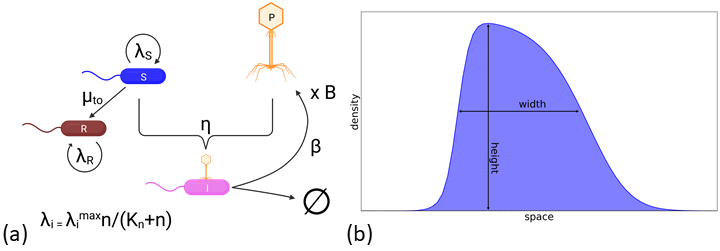
\includegraphics[width=\linewidth]{graphics/2025_09_26_droplets_fig1.png}
\caption{Sketch of the model for bacteria-phage interactions}
\label{fig:model_sketch}
\end{figure}

Our model is most similar to the model used to describe the hitchhiking effect of phages in bacteria~\cite{Ping2020-vd} and is given by the following set of~\gls{pde}s:

\begin{align}
    \frac{\text{d}S}{\text{d}t} = D_b &\frac{\partial^2S}{\partial x^2} + \left( 1 - \mu_{to} \right) \lambda_b S \frac{n}{K_n+n}  - \eta SP \\
    \frac{\text{d}I}{\text{d}t} = D_b &\frac{\partial^2I}{\partial x^2} + \eta SP - \beta I\\
    \frac{\text{d}R}{\text{d}t} = D_r &\frac{\partial^2R}{\partial x^2} + \left[\lambda_r R + \mu_{to} \lambda_b S \right] \frac{n}{K_n+n}\\
    \frac{\text{d}P}{\text{d}t} = D_p &\frac{\partial^2P}{\partial x^2} + \beta BI - \eta P(S+I) \\
    \frac{\text{d}n}{\text{d}t} = D_n &\frac{\partial^2n}{\partial x^2} - \frac{1}{Y} \left( \lambda_b S + \lambda_r R \right) \frac{n}{K_n+n}
\end{align}
where $D_b$, $D_p$ and $D_n$ are the respective diffusion rates, $\mu_{to}$ and $\mu_{back}$ are the towards and backwards mutation rates, $\lambda_S$ and $\lambda_R$ are the respective growth rates, $K_n$ is the half-velocity constant, $\eta$ is the infection rate, $\beta$ is the lysis rate, $B$ is the burst size and $Y$ is the nutrient yield. To improve readability, we omit dependencies on space and time for all variables. The model can easily be generalized to multiple dimensions but we focus here on the most simple one-dimensional case.

These equations can be non-dimensionalized using the following transformations for space, time and quantities:\\
% \begin{align*}
%     x &\rightarrow \tilde{x} = \sqrt{\frac{D_b}{\lambda_b}} x \\
%     t &\rightarrow \tilde{t} = \frac{1}{\lambda_b} \\
%     S &\rightarrow \tilde{S} = K_n Y S \\
%     I &\rightarrow \tilde{I} = K_n Y I \\ 
%     R &\rightarrow \tilde{R} = K_n Y R \\
%     P &\rightarrow \tilde{P} = \frac{\lambda_b}{\eta} P \\
%     n &\rightarrow \tilde{n} = K_n n
% \end{align*}
$x \rightarrow \tilde{x} = \sqrt{\frac{D_b}{\lambda_b}} x$, $t \rightarrow \tilde{t} = \frac{1}{\lambda_b}$, \\
$S \rightarrow \tilde{S} = K_n Y S$, $I \rightarrow \tilde{I} = K_n Y I$, $R \rightarrow \tilde{R} = K_n Y R$, $P \rightarrow \tilde{P} = \frac{\lambda_b}{\eta} P$, $n \rightarrow \tilde{n} = K_n n$\\
Then we can redefine parameters as:\\
% \begin{align*}
%     \tilde{D_p} &= \frac{D_p}{D_b} \\
%     \tilde{D_r} &= \frac{D_r}{D_b} \\
%     \tilde{D_n} &= \frac{D_n}{D_b} \\
%     \tilde{\beta} &= \frac{\beta}{\lambda_b} \\
%     \tilde{\eta} &= \frac{\eta K_n Y}{\lambda_b} \\
%     \tilde{\lambda_r} &= \frac{\lambda_r}{\lambda_b} \\
%     \tilde{B} &= B
% \end{align*}
$\tilde{D_p} = \frac{D_p}{D_b}$, $\tilde{D_r} = \frac{D_r}{D_b}$, $\tilde{D_n} = \frac{D_n}{D_b}$, $\tilde{\beta} = \frac{\beta}{\lambda_b}$, $\tilde{\eta} = \frac{\eta K_n Y}{\lambda_b}$, $\tilde{\lambda_r} = \frac{\lambda_r}{\lambda_b}$, $\tilde{B} = B$\\
and we can write the non-dimensionalized set of coupled~\gls{pde}s, when dropping the tilde, as:
    
\begin{align}
    \frac{\text{d}S}{\text{d}t} &= \frac{\partial^2S}{\partial x^2} + \left( 1 - \mu_{to} \right) S \frac{n}{K_n+n}  - SP \\
    \frac{\text{d}I}{\text{d}t} &= \frac{\partial^2I}{\partial x^2} + SP - \beta I\\
    \frac{\text{d}R}{\text{d}t} &= D_r \frac{\partial^2R}{\partial x^2} + \left[\lambda_r R + \mu_{to} S \right] \frac{n}{K_n+n}\\
    \frac{\text{d}P}{\text{d}t} &= D_p \frac{\partial^2P}{\partial x^2} + \beta \eta BI - \eta P(S+I) \\
    \frac{\text{d}n}{\text{d}t} &= D_n \frac{\partial^2n}{\partial x^2} - \left( S + \lambda_r R \right) \frac{n}{K_n+n}
\end{align}


Numerical simulations of the equations were performed in python, using \text{scipy.solve\_ivp()} with a flexible time step.

For the well-mixed scenario, we drop the diffusion terms, add chemostat balancing terms and after analogous non-dimensionalization, we obtain the following set of~\gls{ode}s:

\begin{align}
    \frac{\text{d}S}{\text{d}t} &= \left( 1 - \mu_{to} \right) S \frac{n}{K_n+n}  - SP - d S\\
    \frac{\text{d}I}{\text{d}t} &= SP - \beta I - d I\\
    \frac{\text{d}R}{\text{d}t} &= \left[\lambda_r R + \mu_{to} S \right] \frac{n}{K_n+n} - d R\\
    \frac{\text{d}P}{\text{d}t} &= \beta \eta BI - \eta P(S+I) -d P\\
    \frac{\text{d}n}{\text{d}t} &= - \left( S + \lambda_r R \right) \frac{n}{K_n+n} - d n
\end{align}

\section{Observables}

We describe and quantify the dynamics being created by solving our model system using three observables for the forming traveling wave. Firstmost, we measure the amount of bacteria which is represented as the area under the curve and additionally we measure the height and the width at 1e-6 of the maximum of the curve as represented in Figure~\ref{fig:model_sketch}b.
